\documentclass[hyperref=unicode, presentation]{beamer}

\usepackage[absolute,overlay]{textpos}
\usepackage{graphicx}
\usepackage{tabularx}
\usepackage{adjustbox}
\usepackage{ucs}
\usepackage[utf8]{inputenc}
%\usepackage{textcomp}
\PrerenderUnicode{ěščřžýáíéĚŠČŘŽÝÁÍÉďťňĎŤŇůúÚóÓ}

\usepackage[czech]{babel}
\mode<presentation>{\usetheme{default}}

 \usecolortheme{crane}
 
 
\adjustboxset*{center}

\mode<presentation>{\usetheme{default}}
\DefineNamedColor{named}{pozadi}{RGB}{200,200,200}
\usecolortheme{crane}

\setbeamertemplate{footline}[frame number]

\addtobeamertemplate{frametitle}{
   \let\insertframetitle\insertsectionhead}{}
\addtobeamertemplate{frametitle}{
   \let\insertframesubtitle\insertsubsectionhead}{}

\makeatletter
  \CheckCommand*\beamer@checkframetitle{\@ifnextchar\bgroup\beamer@inlineframetitle{}}
  \renewcommand*\beamer@checkframetitle{\global\let\beamer@frametitle\relax\@ifnextchar\bgroup\beamer@inlineframetitle{}}
\makeatother
\setbeamercolor{section in toc}{fg=blue}
\setbeamertemplate{section in toc shaded}[default][100]

\usepackage[czech]{babel}
\usepackage[T1]{fontenc}
\usepackage{lmodern}
\usepackage[version=4]{mhchem} 
\begin{document}
\title[Crisis] % (optional, only for long titles)
{C6250 Metody chemického výzkumu - praktikum}

\subtitle{Infračervená a NMR spektroskopie}

\author % (optional, for multiple authors)
{Zdeněk Moravec}

\date[KPT 2004] % (optional)

\frame{\titlepage}

% snimek s cili (zadanim) prace


\section{Průběh cvičení}
\frame{
	\frametitle{}
	\vfill
	\href{https://docs.google.com/spreadsheets/d/1izDYdwXzwPtQ4eQQNLqr0kmJblElyLACq6_Hy9QPg7c/edit\#gid=0}{\emph{Kliknutím na tento text se dostanete do formuláře, kde si můžete zvolit datum konání cvičení.}}
	\\
	\rule{\textwidth}{2pt}
	\\
	Cvičení probíhá v laboratořích A12/112 a A8/1S16. Začátek je v laboratoři A12/112. Doba cvičení je 4-5 hodin.
	\begin{enumerate}
	\item Krátký úvod k IR spektroskopii \textit{(A12/112)}
	\item Spuštění spektrometrů, stanovení vlhkosti uvnitř přístroje
	\item Měření IR spekter vzorků v KBr tabletách a metodou ATR
	\item Interpretace IR spekter
	\item Krátký úvod k NMR spektroskopii \textit{(A8/1S16)}
	\item Měření NMR spekter na benchtop NMR spektrometrech Magritek 60~MHz a Bruker Avance III 300~MHz
	\item Interpretace NMR spekter
	\end{enumerate}
	\vfill
}

\section{Protokol}
\frame{
	\frametitle{}
	\vfill
	\begin{enumerate}
	\item Hlavička (Jméno, datum konání cvičení)
	\item Princip
	\item Postup
	\item Spektra (naměřená spektra studenti dostanou v textovém formátu)
	\item Interpretace spekter
	\item Závěr
	\end{enumerate}
	\hrule
	\begin{itemize}
		\item Protokol zašlete na adresu hugo@chemi.muni.cz do dvou týdnů ode dne konání cvičení.
	\end{itemize}
	\vfill
}

\section{Měření IR spekter vzorků v suspenzi v KBr tabletách}
\frame{
	\frametitle{}
	\vfill
	1-3 mg vzorku smícháme s cca 300 mg KBr a směs rozetřeme v~achátové třecí misce. Získaný prášek nasypeme do lisovací matrice a lisujeme pod tlakem 7-9 tun po dobu cca 1 minuty.
	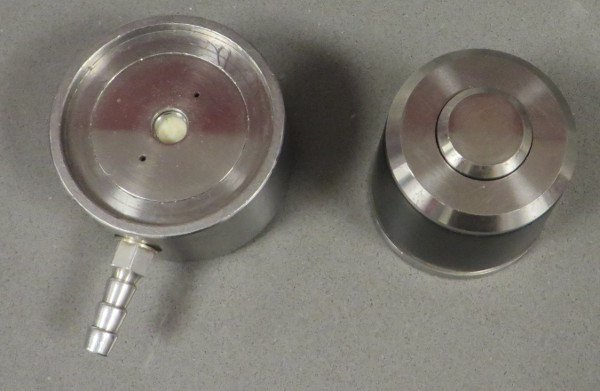
\includegraphics[keepaspectratio,height=3cm]{img/KBr2.jpg}
	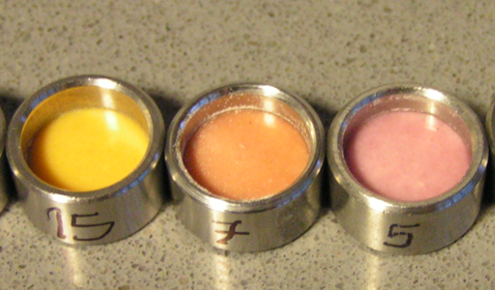
\includegraphics[keepaspectratio,height=3cm]{img/kbr-pellets.png}
	\vfill
}

\section{Měření IR spekter vzorků metodou ATR}
\frame{
	\frametitle{}
	\vfill
	Vzorek nasypeme na krystal diamantu, přitlačíme hrotem a změříme spektrum. Není potřeba vzorky žádným způsobem upravovat.
	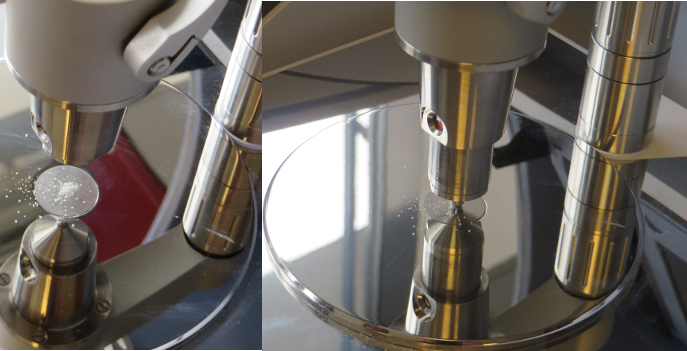
\includegraphics[keepaspectratio,width=10cm]{img/atr.png}
	\vfill
}

\section{NMR}
\frame{
	\frametitle{}
	\vfill
	\begin{itemize}
	\item Měření bude probíhat na spektrometrech Magritek 60~MHz, Bruker Avance III 300~MHz a Bruker Avance III HD 500~MHz.
	\item Cílem měření bude demonstrace vlivu síly magnetického pole na rozlišení NMR spektra a ukázka interpretace 1D a 2D spekter jednoduchých organických sloučenin.
\end{itemize}
	\begin{center}
		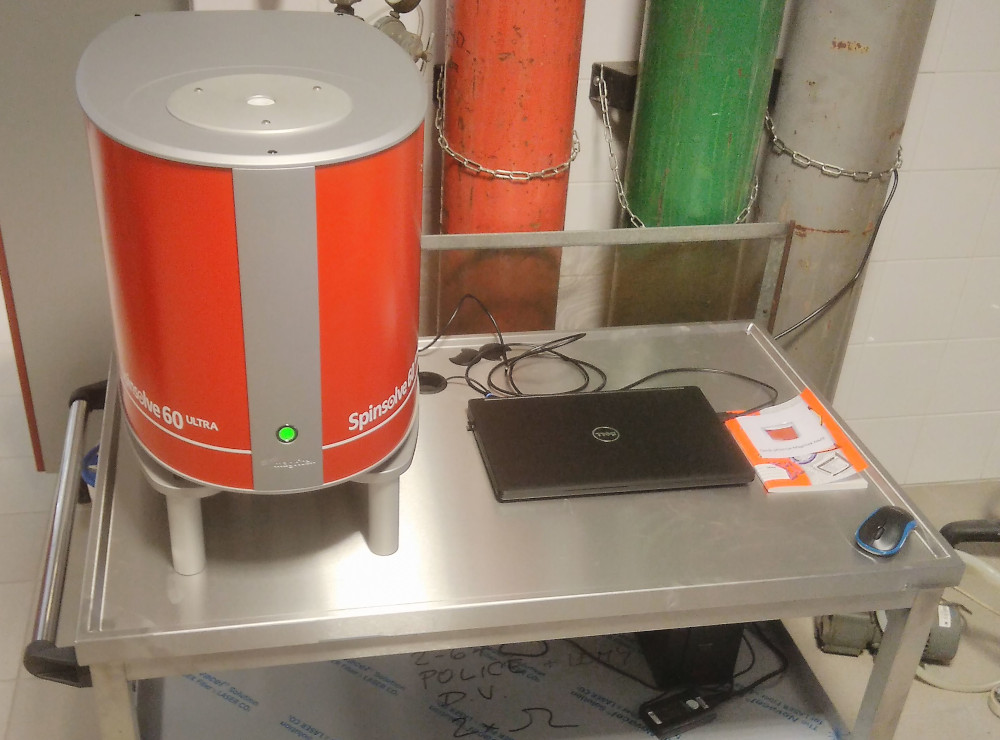
\includegraphics[keepaspectratio,height=4cm]{img/Magritek.jpg}
		\includegraphics[keepaspectratio,height=4cm]{img/NMR300.jpg}
	\end{center}
	\vfill
}

\section{Kontakt}
\frame{
	\frametitle{}
	\vfill
	Pokud budete chtít měřit vlastní vzorky nebo budete mít námět na úpravu průběhu cvičení, napište mi s předstihem.
	\begin{itemize}
	\item Zdeněk Moravec
	\item \url{hugo@chemi.muni.cz}
	\item Tel.: 5 4949 3764
	\item UKB A12/316
	\end{itemize}
	\vfill
}

\end{document}
